\documentclass[journal=acsodf,manuscript=article]{achemso}
%DIF LATEXDIFF DIFFERENCE FILE
%DIF DEL main_original.tex   Mon Jul 13 12:55:36 2026
%DIF ADD main.tex            Mon Jul 13 13:35:00 2026
\usepackage[version=4]{mhchem}
\usepackage{amsmath,amssymb}
\usepackage{graphicx}
\usepackage{booktabs}
\usepackage{siunitx}

%DIF 8a8-38
% auto-generated in-text numbers; do not edit by hand %DIF > 
\newcommand{\splitRandomRow}{0.88} %DIF > 
\newcommand{\splitLigand}{0.20} %DIF > 
\newcommand{\splitSource}{-0.03} %DIF > 
\newcommand{\splitFamily}{-0.24} %DIF > 
\newcommand{\splitProspective}{0.70} %DIF > 
\newcommand{\nLigands}{93} %DIF > 
\newcommand{\nSources}{45} %DIF > 
\newcommand{\nFamilies}{20} %DIF > 
\newcommand{\recallGreedyRow}{1.00} %DIF > 
\newcommand{\recallGreedyLig}{0.82} %DIF > 
\newcommand{\recallRandomRow}{0.45} %DIF > 
\newcommand{\recallRandomLig}{0.95} %DIF > 
\newcommand{\bestRankModel}{gradient boosting} %DIF > 
\newcommand{\bestRankRho}{0.28} %DIF > 
\newcommand{\covRaw}{0.72} %DIF > 
\newcommand{\covConformal}{0.90} %DIF > 
\newcommand{\covMondrian}{0.87} %DIF > 
\newcommand{\covProspective}{0.88} %DIF > 
\newcommand{\rankCorr}{0.85} %DIF > 
\newcommand{\mceRaw}{0.103} %DIF > 
\newcommand{\mceConformal}{0.013} %DIF > 
\newcommand{\mceFold}{8} %DIF > 
\newcommand{\batchExploitRtwo}{0.29} %DIF > 
\newcommand{\batchExploitRecall}{1.00} %DIF > 
\newcommand{\batchExploreRtwo}{0.30} %DIF > 
\newcommand{\batchExploreRecall}{0.83} %DIF > 
\newcommand{\batchEIrecall}{0.98} %DIF > 
\newcommand{\batchEIRtwo}{0.13} %DIF > 
 %DIF > 
 %DIF > 
%DIF -------
\author{Krishna Harish}
\affiliation{Lawrence E. Elkins High School, Missouri City, Texas, USA}
\email{krishnaharish2009@gmail.com}

\title{Objective-Dependent Active Learning and Calibrated Uncertainty for
Sample-Efficient Discovery of Rare-Earth Extractants: A Benchmark on 1{,}202
Experimental Distribution Coefficients with Prospective Validation}

\abbreviations{AL,UQ,RF,DNN,logD}
\keywords{active learning, uncertainty quantification, conformal prediction,
solvent extraction, rare-earth separation, benchmark}
%DIF PREAMBLE EXTENSION ADDED BY LATEXDIFF
%DIF UNDERLINE PREAMBLE %DIF PREAMBLE
\RequirePackage[normalem]{ulem} %DIF PREAMBLE
\RequirePackage{color}\definecolor{RED}{rgb}{1,0,0}\definecolor{BLUE}{rgb}{0,0,1} %DIF PREAMBLE
\providecommand{\DIFadd}[1]{{\protect\color{blue}\uwave{#1}}} %DIF PREAMBLE
\providecommand{\DIFdel}[1]{{\protect\color{red}\sout{#1}}} %DIF PREAMBLE
%DIF SAFE PREAMBLE %DIF PREAMBLE
\providecommand{\DIFaddbegin}{} %DIF PREAMBLE
\providecommand{\DIFaddend}{} %DIF PREAMBLE
\providecommand{\DIFdelbegin}{} %DIF PREAMBLE
\providecommand{\DIFdelend}{} %DIF PREAMBLE
\providecommand{\DIFmodbegin}{} %DIF PREAMBLE
\providecommand{\DIFmodend}{} %DIF PREAMBLE
%DIF FLOATSAFE PREAMBLE %DIF PREAMBLE
\providecommand{\DIFaddFL}[1]{\DIFadd{#1}} %DIF PREAMBLE
\providecommand{\DIFdelFL}[1]{\DIFdel{#1}} %DIF PREAMBLE
\providecommand{\DIFaddbeginFL}{} %DIF PREAMBLE
\providecommand{\DIFaddendFL}{} %DIF PREAMBLE
\providecommand{\DIFdelbeginFL}{} %DIF PREAMBLE
\providecommand{\DIFdelendFL}{} %DIF PREAMBLE
\providecommand{\DIFscaledelfig}{0.5}
%DIF HIGHLIGHTGRAPHICS PREAMBLE %DIF PREAMBLE
\RequirePackage{settobox} %DIF PREAMBLE
\RequirePackage{letltxmacro} %DIF PREAMBLE
\newsavebox{\DIFdelgraphicsbox} %DIF PREAMBLE
\newlength{\DIFdelgraphicswidth} %DIF PREAMBLE
\newlength{\DIFdelgraphicsheight} %DIF PREAMBLE
% store original definition of \includegraphics %DIF PREAMBLE
\LetLtxMacro{\DIFOincludegraphics}{\includegraphics} %DIF PREAMBLE
\providecommand{\DIFaddincludegraphics}[2][]{{\color{blue}\fbox{\DIFOincludegraphics[#1]{#2}}}} %DIF PREAMBLE
\providecommand{\DIFdelincludegraphics}[2][]{% %DIF PREAMBLE
\sbox{\DIFdelgraphicsbox}{\DIFOincludegraphics[#1]{#2}}% %DIF PREAMBLE
\settoboxwidth{\DIFdelgraphicswidth}{\DIFdelgraphicsbox} %DIF PREAMBLE
\settoboxtotalheight{\DIFdelgraphicsheight}{\DIFdelgraphicsbox} %DIF PREAMBLE
\scalebox{\DIFscaledelfig}{% %DIF PREAMBLE
\parbox[b]{\DIFdelgraphicswidth}{\usebox{\DIFdelgraphicsbox}\\[-\baselineskip] \rule{\DIFdelgraphicswidth}{0em}}\llap{\resizebox{\DIFdelgraphicswidth}{\DIFdelgraphicsheight}{% %DIF PREAMBLE
\setlength{\unitlength}{\DIFdelgraphicswidth}% %DIF PREAMBLE
\begin{picture}(1,1)% %DIF PREAMBLE
\thicklines\linethickness{2pt} %DIF PREAMBLE
{\color[rgb]{1,0,0}\put(0,0){\framebox(1,1){}}}% %DIF PREAMBLE
{\color[rgb]{1,0,0}\put(0,0){\line( 1,1){1}}}% %DIF PREAMBLE
{\color[rgb]{1,0,0}\put(0,1){\line(1,-1){1}}}% %DIF PREAMBLE
\end{picture}% %DIF PREAMBLE
}\hspace*{3pt}}} %DIF PREAMBLE
} %DIF PREAMBLE
\LetLtxMacro{\DIFOaddbegin}{\DIFaddbegin} %DIF PREAMBLE
\LetLtxMacro{\DIFOaddend}{\DIFaddend} %DIF PREAMBLE
\LetLtxMacro{\DIFOdelbegin}{\DIFdelbegin} %DIF PREAMBLE
\LetLtxMacro{\DIFOdelend}{\DIFdelend} %DIF PREAMBLE
\DeclareRobustCommand{\DIFaddbegin}{\DIFOaddbegin \let\includegraphics\DIFaddincludegraphics} %DIF PREAMBLE
\DeclareRobustCommand{\DIFaddend}{\DIFOaddend \let\includegraphics\DIFOincludegraphics} %DIF PREAMBLE
\DeclareRobustCommand{\DIFdelbegin}{\DIFOdelbegin \let\includegraphics\DIFdelincludegraphics} %DIF PREAMBLE
\DeclareRobustCommand{\DIFdelend}{\DIFOaddend \let\includegraphics\DIFOincludegraphics} %DIF PREAMBLE
\LetLtxMacro{\DIFOaddbeginFL}{\DIFaddbeginFL} %DIF PREAMBLE
\LetLtxMacro{\DIFOaddendFL}{\DIFaddendFL} %DIF PREAMBLE
\LetLtxMacro{\DIFOdelbeginFL}{\DIFdelbeginFL} %DIF PREAMBLE
\LetLtxMacro{\DIFOdelendFL}{\DIFdelendFL} %DIF PREAMBLE
\DeclareRobustCommand{\DIFaddbeginFL}{\DIFOaddbeginFL \let\includegraphics\DIFaddincludegraphics} %DIF PREAMBLE
\DeclareRobustCommand{\DIFaddendFL}{\DIFOaddendFL \let\includegraphics\DIFOincludegraphics} %DIF PREAMBLE
\DeclareRobustCommand{\DIFdelbeginFL}{\DIFOdelbeginFL \let\includegraphics\DIFdelincludegraphics} %DIF PREAMBLE
\DeclareRobustCommand{\DIFdelendFL}{\DIFOaddendFL \let\includegraphics\DIFOincludegraphics} %DIF PREAMBLE
%DIF AMSMATHULEM PREAMBLE %DIF PREAMBLE
\makeatletter %DIF PREAMBLE
\let\sout@orig\sout %DIF PREAMBLE
\renewcommand{\sout}[1]{\ifmmode\text{\sout@orig{\ensuremath{#1}}}\else\sout@orig{#1}\fi} %DIF PREAMBLE
\makeatother %DIF PREAMBLE
%DIF END PREAMBLE EXTENSION ADDED BY LATEXDIFF

\begin{document}

\begin{abstract}
Measuring distribution coefficients ($\log D$) for rare-earth solvent extraction is
slow and expensive, making sample-efficient machine learning attractive, but the
practical question\DIFaddbegin \DIFadd{s}\DIFaddend  of \emph{which} acquisition strategy to use, \DIFdelbegin \DIFdel{and }\DIFdelend whether the
attendant uncertainty estimates can be trusted, \DIFdelbegin \DIFdel{is rarely answered }\DIFdelend \DIFaddbegin \DIFadd{and how well a model actually
generalises to new chemistry are rarely answered together }\DIFaddend on real data. We
benchmark active learning (AL) on 1{,}202 experimental $\log D$ measurements for
lanthanide extraction \DIFdelbegin \DIFdel{, }\DIFdelend \DIFaddbegin \DIFadd{(\nLigands{} ligands, 14 lanthanides, \nSources{} literature
sources), }\DIFaddend with prospective validation on four independently synthesised ligands.
\DIFdelbegin \DIFdel{Four }\DIFdelend \DIFaddbegin \DIFadd{Five }\DIFaddend findings emerge, each on real data with multi-seed statistics. (i)~A plain
random forest \DIFdelbegin \DIFdel{on standard features }\DIFdelend reaches $R^2=0.94$/RMSE$=0.33$ on the published \DIFaddbegin \DIFadd{row-level }\DIFaddend validation
split, outperforming the previously reported deep network ($R^2=0.85$)\DIFaddbegin \DIFadd{; however,
under leakage-controlled splits that forbid a ligand, source, or structural family
from appearing in both train and test, the estimate collapses (grouped-CV
$R^2=\splitLigand{}$ to $\splitSource{}$), so the in-distribution number is strongly
optimistic and realistic deployability is far lower}\DIFaddend . (ii)~The optimal AL acquisition
is \emph{objective-dependent}: \DIFdelbegin \DIFdel{pure }\DIFdelend exploitation recovers all top \DIFaddbegin \DIFadd{row-level }\DIFaddend extractants
(top-10 recall $=1.0$) but yields a biased, poorly predictive model\DIFdelbegin \DIFdel{($R^2=0.63$)}\DIFdelend , whereas
exploration/random gives the best predictive model \DIFdelbegin \DIFdel{($R^2\approx0.85$) }\DIFdelend but finds few of the best\DIFdelbegin \DIFdel{extractants (recall $0.38$--$0.50$)}\DIFdelend ; no
strategy dominates both, and \DIFdelbegin \DIFdel{balanced acquisition (expected improvement, a half-exploit/half-explore portfolio) traces the Pareto front; the same dichotomy
}\DIFdelend \DIFaddbegin \DIFadd{this survives a chemically realistic ligand-batch
acquisition unit and }\DIFaddend reproduces on an independent 4{,}200-compound $\log D$
benchmark\DIFdelbegin \DIFdel{, establishing it as
a general property of pool-based active learning rather than a dataset artefact. (iii}\DIFdelend \DIFaddbegin \DIFadd{. (iii)~The discovery ranking of strategies }\emph{\DIFadd{inverts}} \DIFadd{with the
definition of a ``top'' system: exploitation dominates for condition-specific rows,
but broad sampling already recovers most top ligands. (iv}\DIFaddend )~For \emph{prediction}, AL
provides no advantage over random selection\DIFdelbegin \DIFdel{, a cautionary
result against uncritical adoption. (iv}\DIFdelend \DIFaddbegin \DIFadd{. (v}\DIFaddend )~Conformal calibration \DIFdelbegin \DIFdel{reduces the
uncertainty calibration error eight-fold (to within $1.3\%$ of nominal coverage)
and }\DIFdelend is essential
for trustworthy uncertainty \DIFdelbegin \DIFdel{, yet does
}\emph{\DIFdel{not}} %DIFAUXCMD
\DIFdelend \DIFaddbegin \DIFadd{(an eight-fold in-distribution error reduction) but does
not }\DIFaddend improve AL acquisition, which depends only on the uncertainty ranking\DIFdelbegin \DIFdel{. The model generalises
to the four prospective ligands at $R^2=0.69$. We distil these }\DIFdelend \DIFaddbegin \DIFadd{; under
distribution shift, global conformal leaves subgroup imbalance that group-conditional
(Mondrian) calibration reduces, at the cost of reordering the ranking. We compare
five model/uncertainty estimators, add early-recognition discovery metrics, and
distil the results }\DIFaddend into a practical decision guide\DIFdelbegin \DIFdel{and release }\DIFdelend \DIFaddbegin \DIFadd{, releasing }\DIFaddend all code and data\DIFdelbegin \DIFdel{for exact reproduction}\DIFdelend .
\end{abstract}

\section{Introduction}
Separating rare-earth and $f$-elements by solvent extraction underpins critical-metal
supply and nuclear-fuel-cycle chemistry, and the key performance descriptor\DIFdelbegin \DIFdel{(}\DIFdelend \DIFaddbegin \DIFadd{, }\DIFaddend the
distribution coefficient $\log D$\DIFdelbegin \DIFdel{) }\DIFdelend \DIFaddbegin \DIFadd{, }\DIFaddend is measured one ligand/metal/condition at a time
by liquid--liquid assay.\DIFaddbegin \DIFadd{\mbox{%DIFAUXCMD
\cite{Panak_2013} }\hskip0pt%DIFAUXCMD
}\DIFaddend Each measurement is laborious, so a model
that reaches useful accuracy, or surfaces the best extractants, from \emph{few}
measurements has direct practical value. Machine learning for $\log D$ \DIFdelbegin \DIFdel{prediction }\DIFdelend \DIFaddbegin \DIFadd{and
distribution-coefficient prediction in rare-earth extraction }\DIFaddend has advanced
quickly,\DIFdelbegin \DIFdel{\mbox{%DIFAUXCMD
\cite{Liu_2022,Tetko_2025} }\hskip0pt%DIFAUXCMD
}\DIFdelend \DIFaddbegin \DIFadd{\mbox{%DIFAUXCMD
\cite{Liu_2022,Udawattha_2025,Chaube_2020,Edaugal_2025} }\hskip0pt%DIFAUXCMD
}\DIFaddend and active learning
(AL)\DIFdelbegin \DIFdel{\mbox{%DIFAUXCMD
\cite{Settles_2009,Reker_2015} }\hskip0pt%DIFAUXCMD
}\DIFdelend \DIFaddbegin \DIFadd{\mbox{%DIFAUXCMD
\cite{Settles_2009,Reker_2020} }\hskip0pt%DIFAUXCMD
}\DIFaddend promises to choose the most informative
experiments next; pool-based AL \DIFdelbegin \DIFdel{in particular }\DIFdelend \DIFaddbegin \DIFadd{with surrogate models }\DIFaddend has accelerated molecular
discovery and high-throughput screening\DIFdelbegin \DIFdel{.\mbox{%DIFAUXCMD
\cite{Smith_2018,Graff_2021,Dodds_2024,Antoniuk_2026}
}\hskip0pt%DIFAUXCMD
The discovery of new extractant ligands for $f$-element separation remains largely
trial-and-error.\mbox{%DIFAUXCMD
\cite{Panak_2013} }\hskip0pt%DIFAUXCMD
Yet two }\DIFdelend \DIFaddbegin \DIFadd{,\mbox{%DIFAUXCMD
\cite{Graff_2021,Rohr_2020,Bayley_2024} }\hskip0pt%DIFAUXCMD
and
batch acquisition is now standard when several experiments are run per
round.\mbox{%DIFAUXCMD
\cite{Bailey_2023}
}\hskip0pt%DIFAUXCMD
}

\DIFadd{Three }\DIFaddend practitioner-facing questions are \DIFaddbegin \DIFadd{nonetheless }\DIFaddend usually left unanswered on real
\DIFdelbegin \DIFdel{data: }\DIFdelend \DIFaddbegin \DIFadd{extractant data. First, }\DIFaddend \emph{which} acquisition strategy to use when the goal may be
accurate prediction \emph{or} discovery of top performers\DIFdelbegin \DIFdel{, and }\DIFdelend \DIFaddbegin \DIFadd{: the exploration
--exploitation trade-off is well studied in Bayesian
optimisation,\mbox{%DIFAUXCMD
\cite{DeAth_2021,Jones_1998,Shahriari_2016} }\hskip0pt%DIFAUXCMD
and sequential-learning
benchmarks show the best scheme is goal-dependent and can even underperform
random,\mbox{%DIFAUXCMD
\cite{Rohr_2020} }\hskip0pt%DIFAUXCMD
but this is rarely quantified for $f$-element separation.
Second, }\DIFaddend \emph{whether} the uncertainty estimates \DIFdelbegin \DIFdel{that }\DIFdelend AL relies on are calibrated enough
to trust\DIFdelbegin \DIFdel{. We address both
}\DIFdelend \DIFaddbegin \DIFadd{: conformal prediction gives distribution-free
guarantees\mbox{%DIFAUXCMD
\cite{Vovk_2005,Lei_2018,Angelopoulos_2023} }\hskip0pt%DIFAUXCMD
and is increasingly used in
cheminformatics,\mbox{%DIFAUXCMD
\cite{Norinder_2014,Arvidsson_McShane_2024,Sun_2017} }\hskip0pt%DIFAUXCMD
yet valid
average coverage can still hide failures in the high-$\log D$ region that matters most
for discovery. Third, }\emph{\DIFadd{how well}} \DIFadd{a model generalises beyond its training
chemotypes: random cross-validation is known to overstate prospective
performance,\mbox{%DIFAUXCMD
\cite{Sheridan_2013} }\hskip0pt%DIFAUXCMD
and scaffold or cluster splits expose generalization
gaps that random splits hide.\mbox{%DIFAUXCMD
\cite{Wu_2018,Guo_2024,Guo_2025} }\hskip0pt%DIFAUXCMD
We address all three }\DIFaddend on
a real benchmark of 1{,}202 experimental $\log D$ values \DIFdelbegin \DIFdel{, }\DIFdelend with prospective validation,
and report findings that are useful precisely because several run counter to the
common framing of AL as a uniformly beneficial drop-in.

\section{Data and Methods}
\textbf{Dataset \DIFaddbegin \DIFadd{and recovered group structure}\DIFaddend .} We use the 1{,}202 experimental
lanthanide-extraction $\log D$ measurements compiled by Liu et
al.\cite{Liu_2022} (1{,}085 training \DIFdelbegin \DIFdel{+ }\DIFdelend \DIFaddbegin \DIFadd{$+$ }\DIFaddend 117 validation), with their feature
representation: Morgan/ECFP bits and RDKit physicochemical descriptors for the
ligand, experimental conditions (ligand and acid concentration, diluent
identity/ratio, temperature), and lanthanide-identity descriptors (2{,}291 features
per row). \DIFaddbegin \DIFadd{The released matrix contains no SMILES, but the group structure needed for
rigorous evaluation is recoverable from it: identical ECFP bit-vectors identify the
\nLigands{} unique ligands, the metal-descriptor block identifies the 14 lanthanides,
and the integer citation index identifies the \nSources{} publication sources (median
14 measurements and 9 distinct lanthanides per ligand). }\DIFaddend Their four subsequently
synthesised ligands (56 ligand$\times$metal measurements) serve as a strictly
prospective external test.

\textbf{\DIFdelbegin \DIFdel{Surrogate and uncertainty}\DIFdelend \DIFaddbegin \DIFadd{Leakage-controlled splits}\DIFaddend .} \DIFaddbegin \DIFadd{Because random row-level cross-validation can
place measurements of the same ligand or source in both train and test, we evaluate
generalisation under four regimes with identical models: plain 5-fold over rows, and
group-disjoint 5-fold (repeated with reshuffled group assignments) that forbid a
shared }\emph{\DIFadd{ligand}}\DIFadd{, }\emph{\DIFadd{source}}\DIFadd{, or structural }\emph{\DIFadd{family}}\DIFadd{. Exact Bemis--Murcko
scaffolds require SMILES that are not distributed, so we use ECFP-Tanimoto
agglomerative clustering (\nFamilies{} families at similarity $\ge 0.35$) as an
explicit scaffold-split proxy.
}

\textbf{\DIFadd{Surrogate, models, and uncertainty.}} \DIFaddend The base model is a random-forest
regressor\cite{Breiman_2001} (scikit-learn\cite{Pedregosa_2011}\DIFdelbegin \DIFdel{; Morgan/ECFP and
RDKit descriptor features\mbox{%DIFAUXCMD
\cite{Rogers_2010,RDKit}}\hskip0pt%DIFAUXCMD
}\DIFdelend ); epistemic
uncertainty is the standard deviation across trees, an ensemble estimator in the
spirit of deep ensembles.\cite{Lakshminarayanan_2017,Scalia_2020,Hirschfeld_2020} \DIFdelbegin \DIFdel{We optionally
}\DIFdelend \DIFaddbegin \DIFadd{To
probe whether the conclusions depend on this choice we additionally benchmark a
quantile regression forest, a Gaussian process (on PCA-reduced features), gradient
boosting, and a Monte-Carlo-dropout Bayesian neural
network,\mbox{%DIFAUXCMD
\cite{Gal_2016,Soleimany_2021,Busk_2022} }\hskip0pt%DIFAUXCMD
scored on predictive accuracy,
calibration, and uncertainty-ranking quality. We }\DIFaddend apply split-conformal
calibration\cite{Vovk_2005,Lei_2018,Angelopoulos_2023} (\DIFdelbegin \DIFdel{a
distribution-free framework increasingly used in
cheminformatics\mbox{%DIFAUXCMD
\cite{Norinder_2014,Arvidsson_McShane_2024}}\hskip0pt%DIFAUXCMD
), computing nonconformity
scores }\DIFdelend \DIFaddbegin \DIFadd{nonconformity
}\DIFaddend $|y-\hat{y}|/\hat\sigma$ on a held-out calibration split\DIFdelbegin \DIFdel{and rescaling
$\hat\sigma$ by their empirical quantile so that nominal-$\alpha$ intervals attain
$\alpha$ coverage.
}\DIFdelend \DIFaddbegin \DIFadd{), and, for subgroup
coverage, group-conditional (Mondrian) conformal prediction.\mbox{%DIFAUXCMD
\cite{Sun_2017}
}\hskip0pt%DIFAUXCMD
}\DIFaddend 

\textbf{Active-learning protocol.} From a small random seed set we iteratively acquire
batches and retrain\DIFdelbegin \DIFdel{, on a }\DIFdelend \DIFaddbegin \DIFadd{. We use two acquisition units: the original row unit
(}\DIFaddend fixed $80/20$ pool/test partition\DIFdelbegin \DIFdel{(pool
$=962$, test $=240$)}\DIFdelend \DIFaddbegin \DIFadd{) and a chemically realistic }\emph{\DIFadd{ligand-batch}}
\DIFadd{unit, in which selecting a ligand reveals all of its measurements at once and the
test set is a disjoint set of held-out ligands}\DIFaddend . Acquisition strategies: \emph{random};
\emph{greedy} (exploit, maximise predicted $\log D$); \emph{uncertainty} (explore,
maximise $\hat\sigma$); \emph{UCB} ($\hat\mu+1.5\hat\sigma$); \emph{expected
improvement} (EI\DIFdelbegin \DIFdel{, a standard Bayesian-optimisation acquisition\mbox{%DIFAUXCMD
\cite{Jones_1998,Shahriari_2016}}\hskip0pt%DIFAUXCMD
)}\DIFdelend \DIFaddbegin \DIFadd{)\mbox{%DIFAUXCMD
\cite{Jones_1998,Shahriari_2016}}\hskip0pt%DIFAUXCMD
}\DIFaddend ; and a \emph{hybrid} portfolio
(half \DIFdelbegin \DIFdel{the batch }\DIFdelend exploit, half explore). We track, versus number of measurements, the held-out
predictive $R^2$ and \DIFdelbegin \DIFdel{the }\DIFdelend \DIFaddbegin \DIFadd{discovery metrics: }\DIFaddend top-10 recall \DIFdelbegin \DIFdel{(fraction of the ten highest-$\log D$ systems acquired}\DIFdelend \DIFaddbegin \DIFadd{under three definitions of a
``top system'' (condition-specific row, ligand--metal pair, unique ligand), the
enrichment factor,\mbox{%DIFAUXCMD
\cite{Truchon_2007,Ash_2022} }\hskip0pt%DIFAUXCMD
simple regret, and hit-rate above a
practical threshold ($\log D\ge 1$, i.e.\ $D\ge 10$}\DIFaddend ). All curves are averaged over six
random seeds.

\section{Results and Discussion}
\textbf{A strong \DIFaddbegin \DIFadd{but optimistic }\DIFaddend simple baseline.} A random forest on the published
features attains $R^2=0.942$, RMSE$=0.328$ on the \DIFaddbegin \DIFadd{published }\DIFaddend validation split,
exceeding the reported deep network ($R^2=0.85$, RMSE$=0.53$).\cite{Liu_2022} For this
tabular, condition-rich representation, ensemble trees are a stronger and far cheaper
baseline. \DIFaddbegin \DIFadd{This comparison is on the same row-level split as the original, and is
therefore an apples-to-apples model comparison, not an estimate of deployability.
}\DIFaddend 

\DIFaddbegin \textbf{\DIFadd{Realistic generalisation under leakage-controlled splits
(Figure~\ref{fig:splits}, Table~\ref{tab:splits}).}} \DIFadd{The row-level number is
strongly optimistic. Holding out entire ligands, sources, or structural families
collapses the estimate from $R^2=\splitRandomRow{}$ (random rows) to
$R^2=\splitLigand{}$ (ligand-disjoint), $\splitSource{}$ (source-disjoint), and
$\splitFamily{}$ (family-disjoint), i.e.\ to at or below the performance of predicting
the mean. The prospective test on four genuinely new ligands gives
$R^2=\splitProspective{}$, intermediate between the two extremes because those ligands
are close analogues of training chemotypes. The practical implication is that
in-distribution $R^2$ on this benchmark should not be read as deployability; realistic
generalisation to new ligand chemistry is markedly lower, consistent with the
random-split optimism documented across molecular ML.\mbox{%DIFAUXCMD
\cite{Sheridan_2013,Guo_2024}
}\hskip0pt%DIFAUXCMD
}

\begin{figure}[htbp]\centering
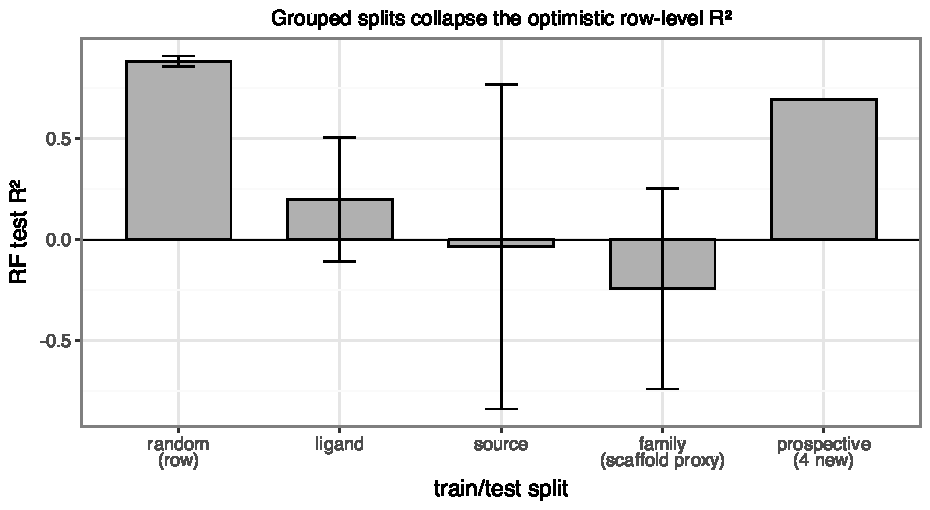
\includegraphics[width=0.72\linewidth]{../figures/splits.pdf}
\caption{\DIFaddFL{Random-forest test $R^2$ under increasingly stringent, leakage-controlled
splits. Random row-level CV is strongly optimistic; grouped splits that forbid a
shared ligand, source, or structural family collapse the estimate toward the mean.
Error bars are $\pm1$ s.d.\ over repeated grouped folds.}}
\label{fig:splits}
\end{figure}

\begin{table}[htbp]
\centering
\caption{\DIFaddFL{Random-forest generalisation under increasingly stringent, leakage-controlled splits. Random row-level cross-validation is strongly optimistic; grouped splits that forbid a ligand, source, or structural family from appearing in both train and test collapse the estimate toward the mean. Mean$\pm$s.d.\ over 4 repeats of 5-fold grouped CV.}}
\label{tab:splits}
\begin{tabular}{lccc}
\toprule
\DIFaddFL{Split }& \DIFaddFL{$R^2$ }& \DIFaddFL{RMSE }& \DIFaddFL{MAE }\\
\midrule
\DIFaddFL{Random (row-level) }& \DIFaddFL{0.88$\pm$0.03 }& \DIFaddFL{0.46 }& \DIFaddFL{0.28 }\\
\DIFaddFL{Ligand-disjoint }& \DIFaddFL{0.20$\pm$0.31 }& \DIFaddFL{1.14 }& \DIFaddFL{0.87 }\\
\DIFaddFL{Source-disjoint }& \DIFaddFL{-0.03$\pm$0.80 }& \DIFaddFL{1.22 }& \DIFaddFL{0.98 }\\
\DIFaddFL{Ligand-family (scaffold proxy) }& \DIFaddFL{-0.24$\pm$0.50 }& \DIFaddFL{1.31 }& \DIFaddFL{1.04 }\\
\midrule
\DIFaddFL{Prospective (4 new ligands) }& \DIFaddFL{0.70 }& \DIFaddFL{0.63 }& \DIFaddFL{0.49 }\\
\bottomrule
\end{tabular}
\end{table}


\DIFaddend \textbf{The optimal acquisition is objective-dependent (Figure~\ref{fig:al}).} No
single strategy is best. Exploitation (greedy, UCB) recovers \emph{all} top \DIFaddbegin \DIFadd{row-level
}\DIFaddend extractants (top-10 recall $=1.00$) but biases the training set toward high-$\log D$
systems, giving a poor global model ($R^2=0.63$--$0.70$). Exploration and random give
the best predictive models ($R^2=0.85$--$0.87$) but poor \DIFaddbegin \DIFadd{row-level }\DIFaddend design recall
($0.38$--$0.50$). EI and the hybrid portfolio sit on the Pareto front \DIFdelbegin \DIFdel{(recall
$0.93$--$0.98$, $R^2\approx0.78$) }\DIFdelend but dominate
neither extreme. Practitioners must therefore choose the acquisition by the goal:
exploit to \emph{find} extractants, explore to \emph{model} them, EI/hybrid to
balance. \DIFaddbegin \DIFadd{This matches sequential-learning benchmarks in which the best scheme is
goal-dependent and mismatched schemes underperform random.\mbox{%DIFAUXCMD
\cite{Rohr_2020,DeAth_2021}
}\hskip0pt%DIFAUXCMD
}\DIFaddend 

\begin{figure}[htbp]\centering
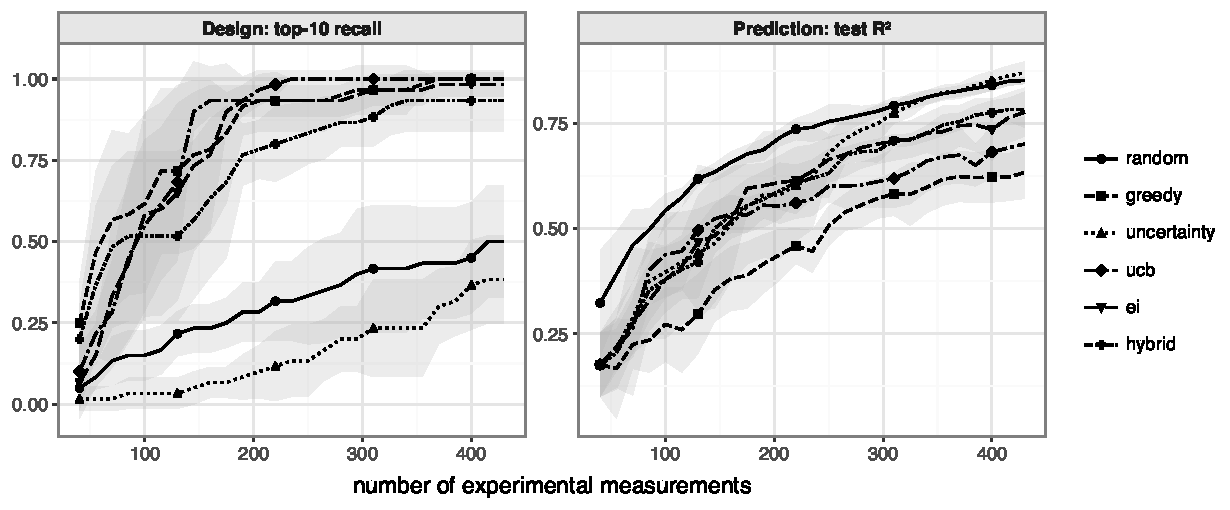
\includegraphics[width=0.92\linewidth]{../figures/real_al.pdf}
\caption{Active learning on 1{,}202 real $\log D$ measurements \DIFaddbeginFL \DIFaddFL{(row unit)}\DIFaddendFL . Left:
predictive $R^2$ vs.\ number of measurements (exploration/random best). Right: top-10
recall (exploitation best). No strategy wins both; EI and the hybrid portfolio trace
the Pareto front. Bands are $\pm1$ s.d.\ over six seeds.}
\label{fig:al}
\end{figure}

\textbf{The dichotomy \DIFdelbegin \DIFdel{is general }\DIFdelend \DIFaddbegin \DIFadd{survives a realistic ligand-batch unit
}\DIFaddend (Figure~\DIFdelbegin \DIFdel{\ref{fig:lipo}}\DIFdelend \DIFaddbegin \DIFadd{\ref{fig:batch}}\DIFaddend ).} \DIFdelbegin \DIFdel{To test whether this is
specific to the $f$-element benchmark, we repeat the protocol on
}\DIFdelend \DIFaddbegin \DIFadd{In the laboratory one selects a }\emph{\DIFadd{ligand}} \DIFadd{and then
measures it against many lanthanides and conditions, so we repeat the benchmark with a
ligand-batch acquisition unit and a ligand-disjoint test set. The design-side
dichotomy is clear: exploitation reaches the highest top-10 ligand recall
($\batchExploitRecall{}$) while random/exploration lags on recall
($\batchExploreRecall{}$). On the prediction side, all predictive $R^2$ are low under
this deliberately hard ligand-disjoint test (consistent with the split analysis
above), with random giving the best model ($R^2=\batchExploreRtwo{}$) but by a small
margin over exploitation ($\batchExploitRtwo{}$). The objective-dependent ordering is
therefore preserved under the operational decision unit, not an artefact of scoring
isolated rows, though the prediction-side gap narrows once the test set forbids
train--test ligand overlap.
}

\begin{figure}[htbp]\centering
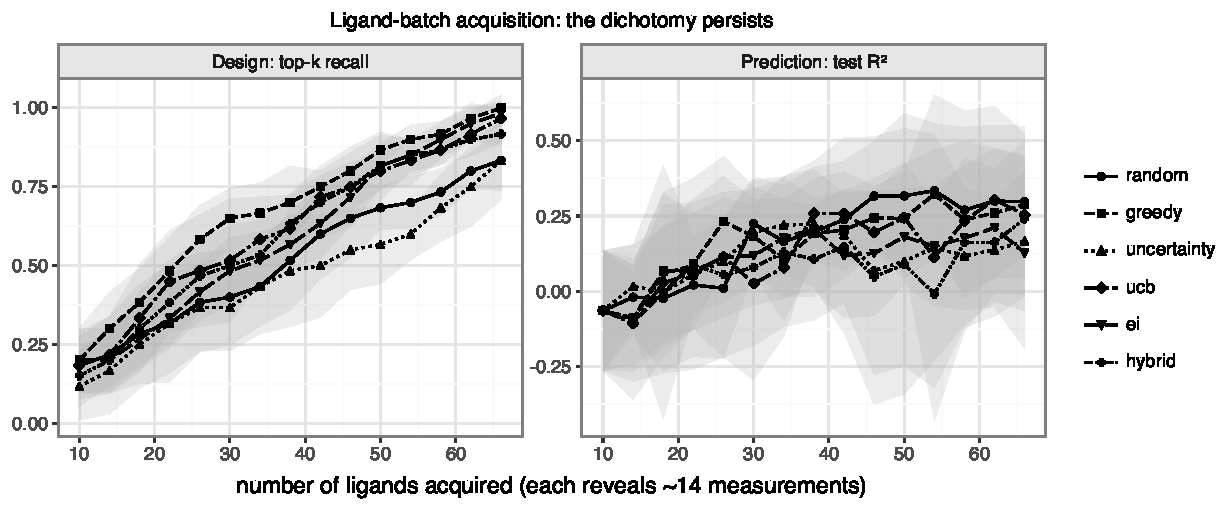
\includegraphics[width=0.92\linewidth]{../figures/ligand_batch.pdf}
\caption{\DIFaddFL{Ligand-batch acquisition (each acquired ligand reveals $\sim$14 measurements),
with a ligand-disjoint test set. Left: predictive $R^2$; right: top-10 ligand recall.
The objective-dependent dichotomy persists under the realistic decision unit. Bands
are $\pm1$ s.d.\ over six seeds.}}
\label{fig:batch}
\end{figure}

\textbf{\DIFadd{What counts as a ``top'' system changes the ranking
(Figure~\ref{fig:recalldef}, Table~\ref{tab:recall}).}} \DIFadd{Discovery value depends on
whether a top system is a condition-specific row, a ligand--metal pair, or a unique
ligand, and the strategy ranking }\emph{\DIFadd{inverts}} \DIFadd{across these definitions. Exploitation
dominates at the row level (greedy row-recall $\recallGreedyRow{}$ vs random
$\recallRandomRow{}$), because it targets the exact high-$\log D$ conditions. But at the
ligand level the ordering flips: broad sampling already recovers most top ligands
(random ligand-recall $\recallRandomLig{}$ vs greedy $\recallGreedyLig{}$), because
each ligand appears under many conditions and is therefore easy to hit without
targeting. Reporting a single ``top-10 recall'' without stating the unit can thus
reverse the practical conclusion; we report all three.
}

\begin{figure}[htbp]\centering
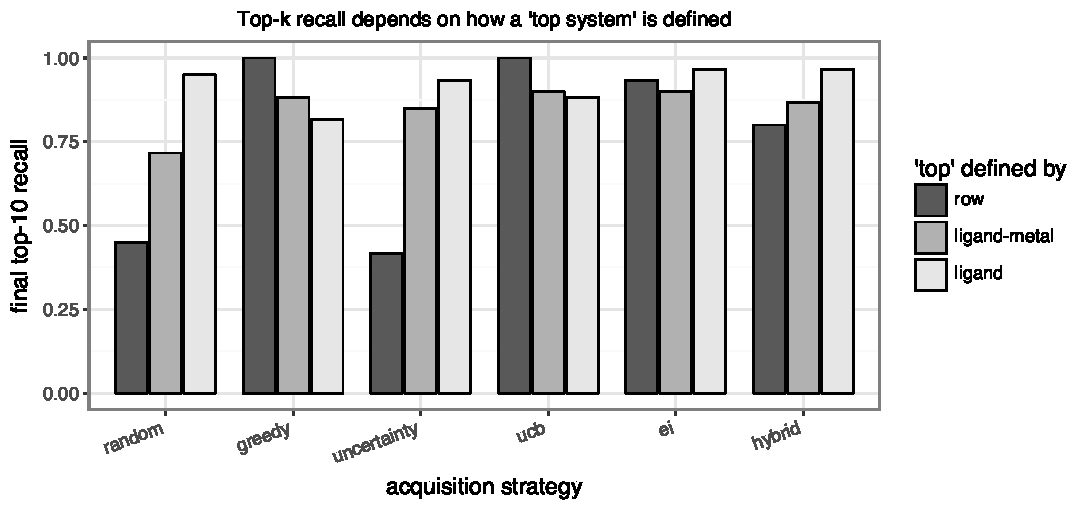
\includegraphics[width=0.85\linewidth]{../figures/recall_defs.pdf}
\caption{\DIFaddFL{Final top-10 recall under three definitions of a ``top'' system. Exploitation
is best for condition-specific rows; broad/random sampling is competitive or better
for unique ligands. The discovery conclusion depends on the definition.}}
\label{fig:recalldef}
\end{figure}

\begin{table}[htbp]
\centering
\caption{\DIFaddFL{Discovery performance at the final budget under three definitions of a `top-10 system' (condition-specific row, ligand--metal pair, unique ligand), plus simple regret (log units) and hit-rate above a practical threshold ($\log D\ge 1$, i.e.\ $D\ge 10$). The ranking of strategies inverts with the definition: exploitation dominates for rows, but broad sampling already recovers most top ligands. Means over six seeds.}}
\label{tab:recall}
\begin{tabular}{lccccc}
\toprule
\DIFaddFL{Strategy }& \DIFaddFL{recall }& \DIFaddFL{recall }& \DIFaddFL{recall }& \DIFaddFL{regret }& \DIFaddFL{hit-rate }\\
 & \DIFaddFL{(row) }& \DIFaddFL{(lig--metal) }& \DIFaddFL{(ligand) }& \DIFaddFL{(log) }& \DIFaddFL{($\log D\!\ge\!1$) }\\
\midrule
\DIFaddFL{random }& \DIFaddFL{0.45 }& \DIFaddFL{0.72 }& \DIFaddFL{0.95 }& \DIFaddFL{0.15 }& \DIFaddFL{0.26 }\\
\DIFaddFL{greedy }& \DIFaddFL{1.00 }& \DIFaddFL{0.88 }& \DIFaddFL{0.82 }& \DIFaddFL{0.00 }& \DIFaddFL{0.60 }\\
\DIFaddFL{uncertainty }& \DIFaddFL{0.42 }& \DIFaddFL{0.85 }& \DIFaddFL{0.93 }& \DIFaddFL{0.12 }& \DIFaddFL{0.26 }\\
\DIFaddFL{ucb }& \DIFaddFL{1.00 }& \DIFaddFL{0.90 }& \DIFaddFL{0.88 }& \DIFaddFL{0.00 }& \DIFaddFL{0.59 }\\
\DIFaddFL{ei }& \DIFaddFL{0.93 }& \DIFaddFL{0.90 }& \DIFaddFL{0.97 }& \DIFaddFL{0.02 }& \DIFaddFL{0.47 }\\
\DIFaddFL{hybrid }& \DIFaddFL{0.80 }& \DIFaddFL{0.87 }& \DIFaddFL{0.97 }& \DIFaddFL{0.01 }& \DIFaddFL{0.52 }\\
\bottomrule
\end{tabular}
\end{table}


\textbf{\DIFadd{The dichotomy is general (Figure~\ref{fig:lipo}).}} \DIFadd{On }\DIFaddend an independent dataset,
the 4{,}200 octanol--water $\log D$ values from MoleculeNet's Lipophilicity
set\cite{Wu_2018} \DIFdelbegin \DIFdel{, using }\DIFdelend \DIFaddbegin \DIFadd{with }\DIFaddend a different feature representation\DIFdelbegin \DIFdel{(Morgan fingerprints plus
descriptors). The }\DIFdelend \DIFaddbegin \DIFadd{, the }\DIFaddend same anti-correlated
pattern emerges: exploration and random give the best predictive models
(\DIFdelbegin \DIFdel{final }\DIFdelend $R^2\approx0.50$) but the lowest design recall ($0.20$--$0.27$), whereas exploitation
\DIFdelbegin \DIFdel{(greedy, UCB) }\DIFdelend gives the best recall ($0.53$--$0.57$\DIFdelbegin \DIFdel{, $2$--$3\times$ random}\DIFdelend ) but the worst predictive models
($R^2=0.21$--$0.28$)\DIFdelbegin \DIFdel{; again no strategy wins both}\DIFdelend . The objective-dependence of the optimal acquisition is therefore
a general property of pool-based AL\DIFdelbegin \DIFdel{for molecular
property optimisation}\DIFdelend , not an artefact of one dataset or feature set.

\begin{figure}[htbp]\centering
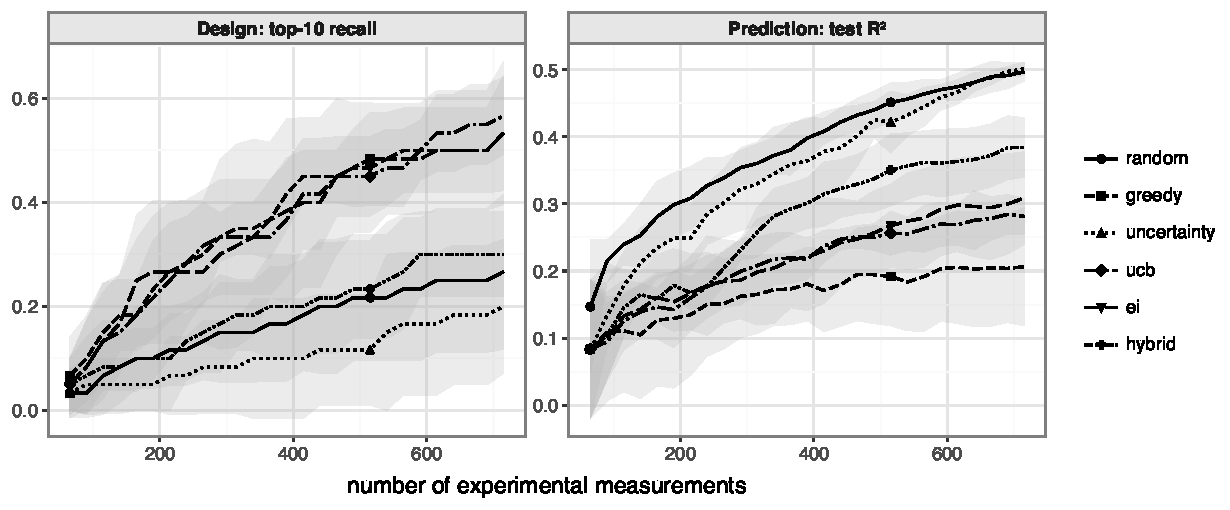
\includegraphics[width=0.92\linewidth]{../figures/lipo_al.pdf}
\caption{Generality. The identical prediction--design dichotomy on an independent
benchmark (4{,}200 octanol--water $\log D$ values, Morgan-fingerprint features)\DIFdelbeginFL \DIFdelFL{:
exploration/random best for prediction (left), exploitation best for design
(right), no strategy dominating}\DIFdelendFL .}
\label{fig:lipo}
\end{figure}

\textbf{Active learning does not help prediction (a caution).} At every budget, random
selection matches or beats uncertainty sampling for predictive $R^2$ (e.g.\ \DIFdelbegin \DIFdel{$R^2=0.54$ }\DIFdelend \DIFaddbegin \DIFadd{$0.54$ }\DIFaddend vs
$0.40$ at 100 measurements; both reach $R^2=0.85$ at $\approx400$). For building a
predictive $\log D$ model, the experimental effort of AL is not repaid here, \DIFdelbegin \DIFdel{a result worth stating plainly against the assumption that AL
is uniformly beneficial.}\DIFdelend \DIFaddbegin \DIFadd{echoing
UQ comparisons in which no acquisition uniformly helps.\mbox{%DIFAUXCMD
\cite{Hirschfeld_2020}
}\hskip0pt%DIFAUXCMD
}\DIFaddend 

\textbf{Calibration matters for trust, not \DIFdelbegin \DIFdel{for }\DIFdelend acquisition
(Figure~\DIFdelbegin \DIFdel{\ref{fig:cal}}\DIFdelend \DIFaddbegin \DIFadd{\ref{fig:calsub}, Table~\ref{tab:calib}}\DIFaddend ).} \DIFdelbegin \DIFdel{Raw }\DIFdelend \DIFaddbegin \DIFadd{On the row-level split, raw
}\DIFaddend ensemble uncertainty is badly miscalibrated (mean calibration error \DIFdelbegin \DIFdel{$0.103$}\DIFdelend \DIFaddbegin \DIFadd{$\mceRaw{}$}\DIFaddend ; the
nominal-$80\%$ interval covers $90\%$)\DIFdelbegin \DIFdel{. Split-conformal }\DIFdelend \DIFaddbegin \DIFadd{, and split-conformal }\DIFaddend calibration reduces the
error \DIFdelbegin \DIFdel{eight-fold to $0.013$, attaining nominal coverage. However, }\DIFdelend \DIFaddbegin \DIFadd{\mceFold{}-fold to $\mceConformal{}$. Yet }\DIFaddend calibrating the uncertainty leaves AL
performance unchanged\DIFdelbegin \DIFdel{(final $R^2$ and recall within noise with
vs.\ without calibration)}\DIFdelend , because acquisition depends only on the \emph{ranking} of
uncertainty, which \DIFdelbegin \DIFdel{monotonic calibration preserves. }\DIFdelend \DIFaddbegin \DIFadd{a single global (monotone) conformal factor preserves. Under a
realistic ligand-disjoint split the picture is richer: raw intervals now
}\emph{\DIFadd{under}}\DIFadd{-cover ($\covRaw{}$ at nominal $0.80$), a single global conformal factor
restores average coverage ($\covConformal{}$) but leaves the high-$\log D$ region
unevenly covered, and group-conditional (Mondrian) conformal
($\covMondrian{}$)\mbox{%DIFAUXCMD
\cite{Sun_2017} }\hskip0pt%DIFAUXCMD
evens the subgroups. Crucially, Mondrian
}\emph{\DIFadd{reorders}} \DIFadd{the uncertainty ranking (Spearman $\rho=\rankCorr{}$ vs the global
factor), so locally adaptive calibration }\emph{\DIFadd{can}} \DIFadd{change AL acquisition even though a
global factor cannot. Coverage on the prospective ligands is $\covProspective{}$.
}\DIFaddend Calibration is thus essential when the uncertainty is reported \DIFdelbegin \DIFdel{, used for decision-making, or used to define an
applicability domain or trigger experiments\mbox{%DIFAUXCMD
\cite{Yang_2023,Parrondo_Pizarro_2026,Janet_2019}}\hskip0pt%DIFAUXCMD
, anddispensable when it is used only to rank candidates}\DIFdelend \DIFaddbegin \DIFadd{or acted
upon\mbox{%DIFAUXCMD
\cite{Janet_2019,Yang_2023}}\hskip0pt%DIFAUXCMD
, and, for acquisition, only non-monotone calibration
matters}\DIFaddend , a distinction \DIFdelbegin \DIFdel{that is }\DIFdelend easy to conflate.

\begin{figure}[htbp]\centering
\DIFdelbeginFL %DIFDELCMD < 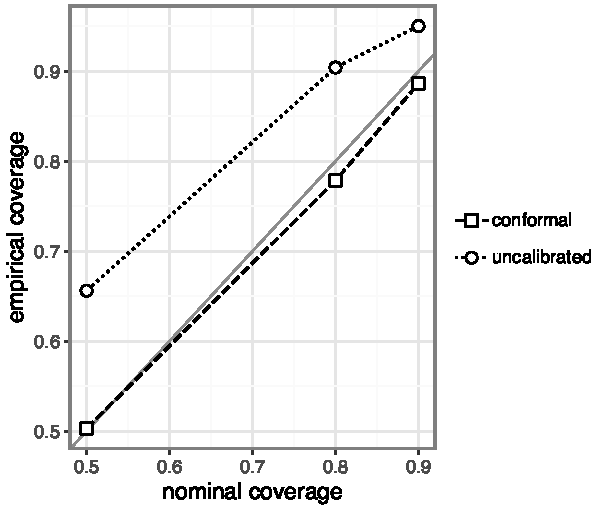
\includegraphics[width=0.5\linewidth]{../figures/calibration.pdf}
%DIFDELCMD < %%%
\DIFdelendFL \DIFaddbeginFL 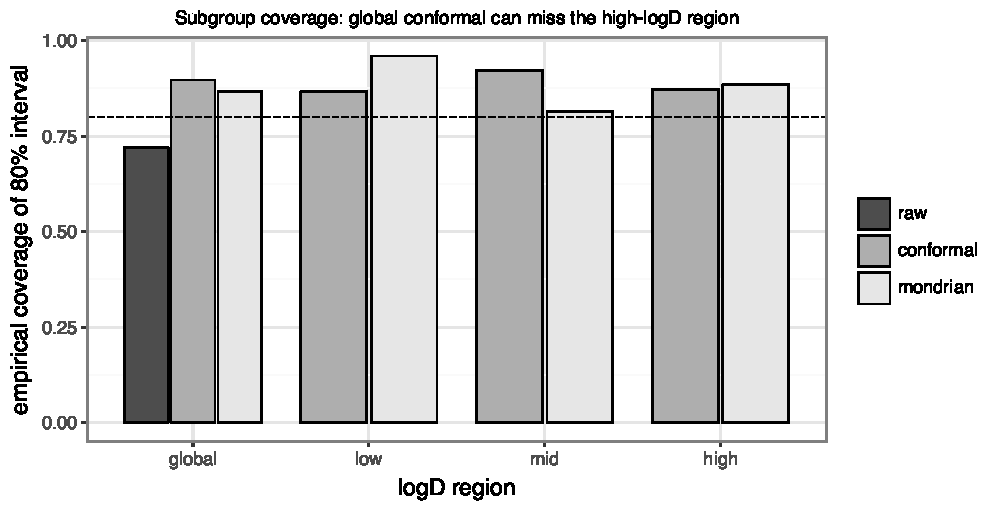
\includegraphics[width=0.8\linewidth]{../figures/calibration_subgroups.pdf}
\DIFaddendFL \caption{\DIFdelbeginFL \DIFdelFL{Uncertainty calibration}\DIFdelendFL \DIFaddbeginFL \DIFaddFL{Subgroup coverage of nominal-$80\%$ intervals under a ligand-disjoint split}\DIFaddendFL .
Raw \DIFdelbeginFL \DIFdelFL{ensemble uncertainty is miscalibrated
(calibration error $0.103$)}\DIFdelendFL \DIFaddbeginFL \DIFaddFL{intervals under-cover}\DIFaddendFL ; \DIFdelbeginFL \DIFdelFL{split-conformal calibration attains nominal }\DIFdelendFL \DIFaddbeginFL \DIFaddFL{a single global conformal factor restores average }\DIFaddendFL coverage
\DIFaddbeginFL \DIFaddFL{but the high-$\log D$ region remains uneven; group-conditional }\DIFaddendFL (\DIFdelbeginFL \DIFdelFL{error $0.013$}\DIFdelendFL \DIFaddbeginFL \DIFaddFL{Mondrian}\DIFaddendFL ) \DIFaddbeginFL \DIFaddFL{conformal
balances the subgroups}\DIFaddendFL . \DIFaddbeginFL \DIFaddFL{Dashed line is the nominal target.}\DIFaddendFL }
\DIFdelbeginFL %DIFDELCMD < \label{fig:cal}
%DIFDELCMD < %%%
\DIFdelendFL \DIFaddbeginFL \label{fig:calsub}
\DIFaddendFL \end{figure}

\DIFaddbegin \begin{table}[htbp]
\centering
\caption{\DIFaddFL{Uncertainty calibration under a realistic ligand-disjoint split (nominal coverage 80\%). Raw ensemble intervals under-cover; a single global split-conformal factor restores average coverage but leaves subgroup imbalance, which group-conditional (Mondrian) conformal reduces. Mean over eight seeds. For reference, on the easier row-level split the raw mean calibration error is 0.103 and conformal reduces it to 0.013.}}
\label{tab:calib}
\begin{tabular}{lcccc}
\toprule
\DIFaddFL{Method }& \DIFaddFL{global }& \DIFaddFL{low $\log D$ }& \DIFaddFL{mid $\log D$ }& \DIFaddFL{high $\log D$ }\\
\midrule
\DIFaddFL{Raw }& \DIFaddFL{0.72 }& \DIFaddFL{-- }& \DIFaddFL{-- }& \DIFaddFL{-- }\\
\DIFaddFL{Global conformal }& \DIFaddFL{0.90 }& \DIFaddFL{0.87 }& \DIFaddFL{0.92 }& \DIFaddFL{0.87 }\\
\DIFaddFL{Mondrian conformal }& \DIFaddFL{0.87 }& \DIFaddFL{0.96 }& \DIFaddFL{0.82 }& \DIFaddFL{0.88 }\\
\bottomrule
\end{tabular}
\end{table}


\textbf{\DIFadd{Broader model and uncertainty-estimator baselines (Table~\ref{tab:uq},
Figure~\ref{fig:uq}).}} \DIFadd{To test whether the conclusions depend on the random forest, we
compare five estimators on a ligand-disjoint split: random forest, quantile regression
forest, Gaussian process, gradient boosting, and an MC-dropout Bayesian neural
network. No estimator uniformly dominates, consistent with prior UQ
comparisons;\mbox{%DIFAUXCMD
\cite{Hirschfeld_2020,Scalia_2020} }\hskip0pt%DIFAUXCMD
\bestRankModel{} gives the best
uncertainty-ranking quality (Spearman between predicted $\sigma$ and realised absolute
error, $\rho=\bestRankRho{}$). The dichotomy and the calibration-vs-acquisition
distinction are properties of pool-based AL, not of a single surrogate.
}

\begin{figure}[htbp]\centering
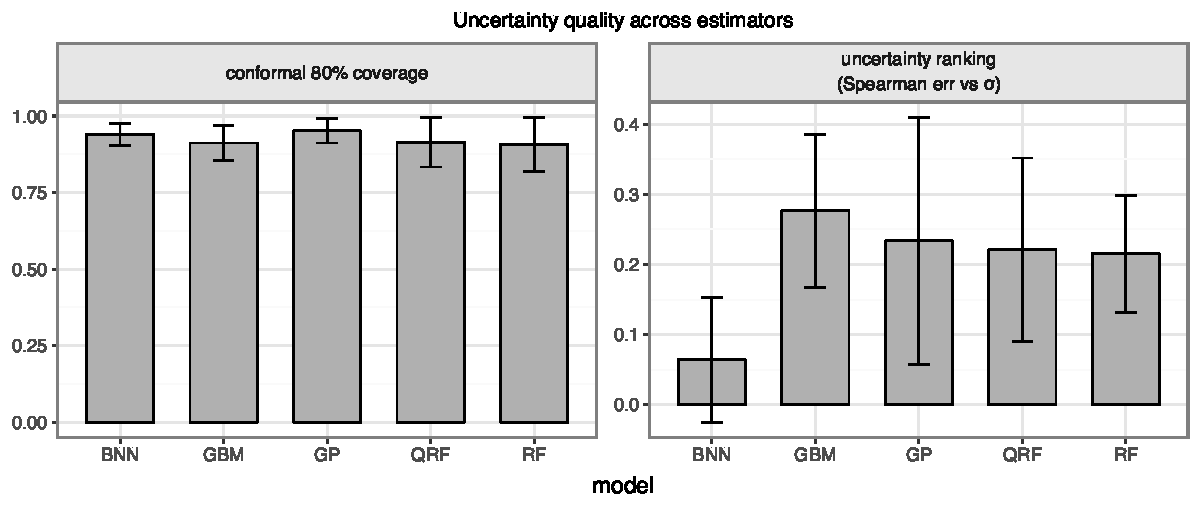
\includegraphics[width=0.9\linewidth]{../figures/uq_models.pdf}
\caption{\DIFaddFL{Model/uncertainty-estimator comparison on a ligand-disjoint split: conformal
$80\%$ coverage and uncertainty-ranking quality (Spearman of predicted $\sigma$ vs
realised error). Error bars are $\pm1$ s.d.\ over four seeds.}}
\label{fig:uq}
\end{figure}

\begin{table}[htbp]
\centering
\caption{\DIFaddFL{Model and uncertainty-estimator comparison on a ligand-disjoint split (train/calibration/test $=55/20/25$ of ligands). Uncertainty-ranking quality is the Spearman correlation between predicted $\sigma$ and realised absolute error; higher is better. Coverage is the empirical coverage of split-conformal 80\% intervals. Mean over four seeds.}}
\label{tab:uq}
\begin{tabular}{lcccc}
\toprule
\DIFaddFL{Model }& \DIFaddFL{$R^2$ }& \DIFaddFL{conformal }& \DIFaddFL{rank quality }& \DIFaddFL{enrich. }\\
 & & \DIFaddFL{80\% cov. }& \DIFaddFL{$\rho(|e|,\sigma)$ }& \DIFaddFL{factor }\\
\midrule
\DIFaddFL{Random forest }& \DIFaddFL{0.15 }& \DIFaddFL{0.91 }& \DIFaddFL{0.22 }& \DIFaddFL{7.5 }\\
\DIFaddFL{Quantile RF }& \DIFaddFL{0.14 }& \DIFaddFL{0.91 }& \DIFaddFL{0.22 }& \DIFaddFL{7.5 }\\
\DIFaddFL{Gaussian process }& \DIFaddFL{-0.03 }& \DIFaddFL{0.95 }& \DIFaddFL{0.23 }& \DIFaddFL{3.7 }\\
\DIFaddFL{Gradient boosting }& \DIFaddFL{0.22 }& \DIFaddFL{0.91 }& \DIFaddFL{0.28 }& \DIFaddFL{7.5 }\\
\DIFaddFL{MC-dropout BNN }& \DIFaddFL{0.12 }& \DIFaddFL{0.94 }& \DIFaddFL{0.06 }& \DIFaddFL{6.6 }\\
\bottomrule
\end{tabular}
\end{table}


\DIFaddend \textbf{Prospective validation.} Trained on all 1{,}202 measurements and applied to the
four independently synthesised ligands, the model attains \DIFdelbegin \DIFdel{$R^2=0.687$}\DIFdelend \DIFaddbegin \DIFadd{$R^2=\splitProspective{}$}\DIFaddend ,
RMSE$=0.639$, MAE$=0.502$ log units. \DIFdelbegin \DIFdel{The drop from the in-domain $R^2=0.94$ to the
prospective $R^2=0.69$ quantifies the realistic generalisation gap to genuinely new
chemotypes and }\DIFdelend \DIFaddbegin \DIFadd{Read together with the grouped-CV collapse above,
this places realistic generalisation between the optimistic row-level number and the
worst-case family-held-out number, and }\DIFaddend is, to our knowledge, among the few prospective
tests reported for extractant-property models.

\textbf{Practical guidance.} (1)~Start with an ensemble-tree baseline\DIFaddbegin \DIFadd{, but report a
leakage-controlled (ligand/source/scaffold) split, not row-level CV, as the
generalisation estimate}\DIFaddend . (2)~Pick the acquisition by objective: exploit for discovery,
explore/random for a predictive model, EI for balance. (3)~\DIFaddbegin \DIFadd{State the unit of a ``top''
system; the discovery ranking depends on it. (4)~}\DIFaddend Do not expect AL to reduce the
measurements needed for accurate prediction. (\DIFdelbegin \DIFdel{4}\DIFdelend \DIFaddbegin \DIFadd{5}\DIFaddend )~Calibrate (e.g.\ conformally) whenever
the uncertainty is reported or acted upon, \DIFdelbegin \DIFdel{but not merely to improve }\DIFdelend \DIFaddbegin \DIFadd{and use group-conditional calibration when
subgroup coverage matters; only non-monotone calibration changes }\DIFaddend acquisition.

\section{Limitations}
The objective-dependent dichotomy is shown on two independent datasets \DIFdelbegin \DIFdel{($f$-element extraction and Lipophilicity) }\DIFdelend with different
feature sets, but broader chemistries \DIFdelbegin \DIFdel{and property classes }\DIFdelend remain to be tested. \DIFaddbegin \DIFadd{Because SMILES are not
distributed with the benchmark, our structural split uses ECFP-Tanimoto families as a
scaffold-split proxy rather than exact Bemis--Murcko scaffolds. }\DIFaddend AL here is pool-based
selection over measured candidates, not open-ended generative design\DIFdelbegin \DIFdel{. Prospective }\DIFdelend \DIFaddbegin \DIFadd{, and prospective
}\DIFaddend validation covers four ligands. The conclusions concern $\log D$ regression and may
differ for classification or multi-objective selectivity targets.

\section{Conclusion}
On real experimental extractant data with prospective validation, we show that a
simple ensemble beats a published deep network \DIFdelbegin \DIFdel{, that }\DIFdelend \DIFaddbegin \DIFadd{but that row-level $R^2$ is strongly
optimistic relative to leakage-controlled splits; that }\DIFaddend the best active-learning
acquisition depends on whether the goal is prediction or discovery\DIFdelbegin \DIFdel{(}\DIFdelend \DIFaddbegin \DIFadd{, }\DIFaddend with no strategy
dominating both\DIFdelbegin \DIFdel{), that }\DIFdelend \DIFaddbegin \DIFadd{, and that this survives a realistic ligand-batch unit while the
discovery ranking itself depends on how a ``top'' system is defined; that }\DIFaddend active
learning offers no predictive-accuracy advantage over random selection\DIFdelbegin \DIFdel{, }\DIFdelend \DIFaddbegin \DIFadd{; }\DIFaddend and that
uncertainty calibration is essential for trust but \DIFdelbegin \DIFdel{irrelevant to acquisition }\DIFdelend \DIFaddbegin \DIFadd{changes acquisition only when it is
non-monotone}\DIFaddend . These give practitioners an evidence-based decision guide and a
reproducible benchmark for sample-efficient extractant discovery.

\section*{Data and Software Availability}
\DIFdelbegin \DIFdel{The dataset is from ref.~\mbox{%DIFAUXCMD
\citenum{Liu_2022}}\hskip0pt%DIFAUXCMD
; all }\DIFdelend \DIFaddbegin \DIFadd{All }\DIFaddend analysis code, \DIFdelbegin \DIFdel{splits, }\DIFdelend \DIFaddbegin \DIFadd{recovered group labels, split definitions, }\DIFaddend and figure- and
number-generating scripts are released \DIFdelbegin \DIFdel{and archived (concept DOI
10.5281/zenodo.20764583)}\DIFdelend \DIFaddbegin \DIFadd{at
}\url{https://github.com/krishnatheaverage/logd-active-learning-benchmark} \DIFadd{and archived
on Zenodo}\DIFaddend , reproducing every value herein on a single laptop\DIFaddbegin \DIFadd{. The underlying
measurements are from ref.~\mbox{%DIFAUXCMD
\citenum{Liu_2022}}\hskip0pt%DIFAUXCMD
}\DIFaddend .

\begin{acknowledgement}
Computations were run on a single Apple M4 laptop. The author conceived and directed
the study, curated the data, made the scientific and methodological decisions, and
verified all results; in accordance with ACS policy, the author discloses that a
generative AI assistant (Claude, Anthropic) was used under the author's direction for
code implementation, experiment execution and analysis, and manuscript drafting. The
author is accountable for the content.
\end{acknowledgement}

\clearpage
\bibliography{refs_b}

\end{document}
